\documentclass[12pt]{report}
\usepackage[utf8]{inputenc}
\usepackage[russian]{babel}
\usepackage{amsmath}
\usepackage{tabularx}
\usepackage{subcaption}
\usepackage{graphicx}
\usepackage{multicol}
\usepackage{floatrow}
\usepackage{indentfirst}
\usepackage[top=0.7in, bottom=0.7in, left=1in, right=1in]{geometry}

\graphicspath{ {/} }

\newenvironment{Figure}
  {\par\medskip\noindent\minipage{\linewidth}}
  {\endminipage\par\medskip}

\begin{document}

\section*{\centering{Лабораторная работа 2.2--2.3 \\
Изучение спектров атома водорода и молекулы йода}}

\textbf{В работе исследуются:} а) сериальные закономерности в оптическом спектре водорода; б) спектр поглощения паров йода в видимой области.

\begin{figure}[h]
    \centering
    \begin{floatrow}
        \ffigbox[\linewidth]
        {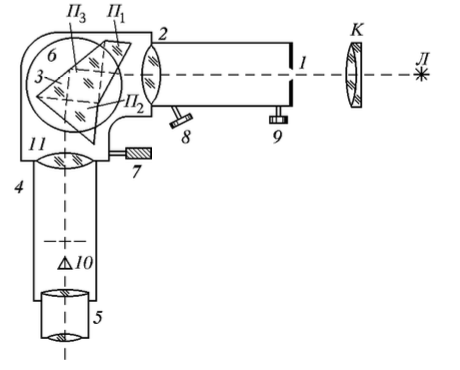
\includegraphics[width=1.0\linewidth]{pic1.png}}
        {\caption{Схема экспериментальной установки для изучения спектра атома водорода}}
    \end{floatrow}
\end{figure}


\subsection*{Теоретические сведения}

Длины волн спектральных линий водородоподобного атома:
\begin{equation}
\label{e1}
\frac{1}{\lambda_{mn}} = RZ^2\left( \frac{1}{n^2} - \frac{1}{m^2} \right),
\end{equation}

где $R$ --- постоянная Ридберга, $m$ и $n$ --- целые числа, $Z$ --- заряд ядра.

Энергия основного состояния электрона:
$$E = -RZ^2$$

Условие, соответствующее $n$-му состоянию электрона:
$$2\pi r = \lambda n,$$

где $r$ --- радиус орбиты.


\subsection*{Ход выполнения и результаты измерений}

\textbf{Задание I. Градуировка спектрометра по спектру неона}

\begin{enumerate}

\item[1.] В первую очередь проградуируем спектрометр по спектру неона.
Для этого сопоставим спектральные линии неона с соответствующими им
длинами волн.

{
    \centering
    \begin{tabularx}{0.937\textwidth}{|X|X|X|X|X|X|X|X|X|}
        \hline
        n & 3 & 4 & 5 & 6 & 7 & 8 & 9 & 10 \\
        \hline
        дел & 2841 & 2830 & 2804 & 2780 & 2772 & 2735 & 2726 & 2708 \\
        \hline
        $\lambda, \mathring{A}$ & 6717 & 6678 & 6599 & 6533 & 6507 & 6402 & 6383 & 6334 \\
        \hline
        \hline
        n & 11 & 12 & 13 & 14 & 15 & 16 & 17 & 18 \\
        \hline
        дел & 2698 & 2682 & 2662 & 2640 & 2630 & 2610 & 2600 & 2582 \\
        \hline
        $\lambda, \mathring{A}$ & 6305 & 6267 & 6217 & 6164 & 6143 & 6096 & 6074 & 6030 \\
        \hline
        \hline
        n & 19 & 20 & 21 & 22 & 23 & 24 & 25 & \\
        \hline
        дел & 2556 & 2541 & 2512 & 2498 & 2240 & 2200 & 2193 & \\
        \hline
        $\lambda, \mathring{A}$ & 5976 & 5945 & 5882 & 5852 & 5401 & 5341 & 5331 & \\
        \hline
    \end{tabularx}
}
\\

Построим градуировочную кривую:

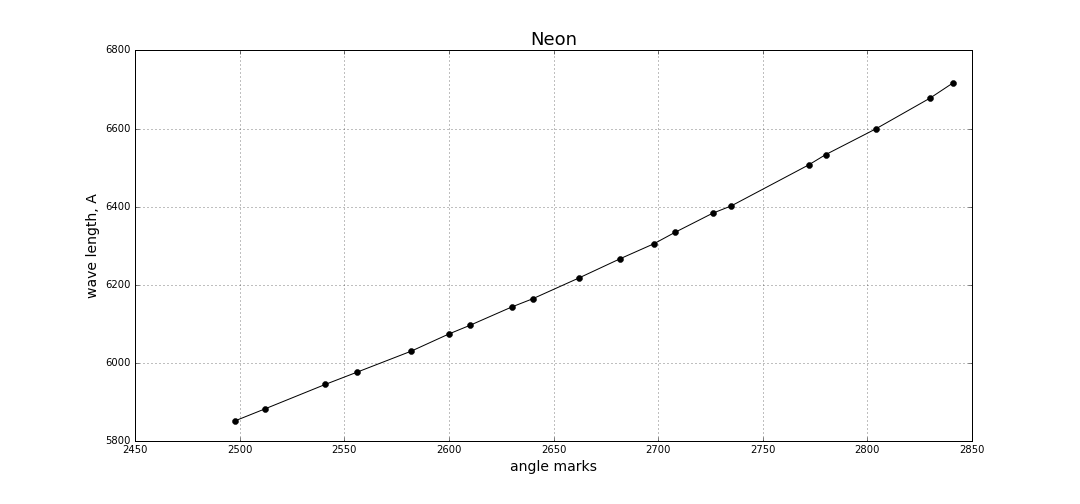
\includegraphics[width=0.94 \textwidth]{g1_neon.png}


\item[2.] Оценим погрешность измерений: для этого измерим
одну и ту же спектральную линию несколько раз.

{
    \centering
    \begin{tabularx}{0.937\textwidth}{|X|X|X|X|X|X|X|X|X|}
        \hline
        № & $n_1$ & $n_2$ & $n_3$ & $n_4$ & $n_5$ & $\overline{n}$ & $\sigma_n$ \\
        \hline
        24 & 2238 & 2238 & 2237 & 2240 & 2240 & \textbf{2239} & 0,6 \\
        \hline
        22 & 2500 & 2496 & 2501 & 2498 & 2496 & \textbf{2498} & 1.02 \\
        \hline
        14 & 2638 & 2640 & 2642 & 2640 & 2636 & \textbf{2639} & 1.02 \\
        \hline
        8 & 2736 & 2734 & 2736 & 2735 & 2736 & \textbf{2735} & 0.4 \\
        \hline
    \end{tabularx}
}
\\
\\

Рассчитаем погрешность по формуле погрешности среднего арифметического (см. таблицу)

\begin{equation}
\label{e2}
    \sigma_{\eta_\text{ср}} = \sqrt{\frac{1}{n(n-1)} \sum\limits_{i=1}^n (\eta_i - \eta_\text{ср})^2}
\end{equation}

\item[3.] Проградуируем спектрометр по спектру ртути:

{
    \centering
    \begin{tabularx}{0.937\textwidth}{|X|X|X|X|X|X|X|X|X|}
        \hline
        n & 6 & 5 & 4 & 3 & 2 & 1 & К1 & К2 \\
        \hline
        дел & 650 & 1190 & 1852 & 2278 & 2455 & 2460 & 2662 & 2902 \\
        \hline
        $\lambda$, нм & 404.7 & 435.8 & 491.6 & 546.1 & 577.0 & 579.1 & 623.4 & 690.7 \\
        \hline
    \end{tabularx}
}
\\
\\

Построим градуировочную кривую:

% \includegraphics[width=0.94 \textwidth]{lab4_2_2_1}


\textbf{Задание II. Спектр водорода}

\item[1.] С помощью построенного калибровочного графика определим длины волн $H_\alpha$, $H_\beta$, $H_\gamma$.

{
    \centering
    \begin{tabularx}{0.937\textwidth}{|X|X|X|X|X|X|X|X|X|}
        \hline
        & $H_\alpha$ & $H_\beta$ & $H_\gamma$ \\
        \hline
        цвет & красная & синяя & фиолетовая \\
        \hline
        дел & 2786 & 1802 & 1160 \\
        \hline
        $\lambda, \mathring{A}$ & 6550 & 4875 & 4350 \\
        \hline
        $R$ 10.99 & 10.94 & 10.95 \\
        \hline
    \end{tabularx}
}
\\
\\
% 1) добавить R

\item[2.] Убедимся, что отношение длин волн водородных линий соответствуют формуле сериальной закономерности \eqref{e1} при $n = 2$.

\item[3.] Для каждой из линий вычислим значение постоянной Ридберга (см. таблицу).

\item[4.] Теперь вычислим погрешность постоянной Ридберга с помощью формулы погрешности среднего арифметического \eqref{e2}.

Итого:
$$R = 10.96 \pm 0.01 \text{ мкм}^{-1}$$

В пределах погрешности реальное и вычисленное значения совпадают.

\textbf{Задание III. Спектр йода}

\item[1.] Определим длины волн линий поглощения йода, соответствующие
делениям барабана монохроматора.

{
    \centering
    \begin{tabularx}{0.937\textwidth}{|X|X|X|X|X|X|X|X|X|}
        \hline
        & $n_{1,0}$ & $n_{1,5}$ & $n_\text{гр}$ \\
        \hline
        дел & 2772 & 2688 & 2030 \\
        \hline
        $\lambda, \mathring{A}$ & 6490 & 6250 & 5125 \\
        \hline
    \end{tabularx}
}
\\
\\

\item[2.] Вычислим энергию колебательного кванта возбужденного состояния
молекулы йода:

$$h\nu_2 = \frac{h\nu_{1,5} - h\nu_{1,0}}{5} = \frac{hc}{5} \left( \frac{1}{\lambda_{1,5}} - \frac{1}{\lambda_{1,0}} \right) = 1467 \cdot 10^{-5} \text{ эВ}$$

\item[3.] Учитывая то, что $h\nu_1 = 0.027$ эВ --- энергия колебательного кванта основного состояния, $E_A = 0.94$ эВ --- энергия возбуждения атома, рассчитаем

а) энергию электронного перехода
$$h\nu_\text{эл} = h\nu_{1,0} + h\nu_{} = h\nu_\text{гр} + h\nu_{} = 2.012 \text{ эВ}$$

б) энергию диссоциации молекулы в основном состоянии
$$D_1 = h\lambda_\text{гр} - E_A = 1.482 \text{ эВ}$$

в) энергию диссоциации молекулы в возбужденном состоянии
$$D_2 = h\lambda_\text{гр} - h\lambda_\text{эл} = 0.413 \text{ эВ}$$

\item[4.] Сравним полученные значения с достоверными $h\nu_\text{гр} = 2.440$ и $D_1 = 1.500$ и получим погрешности $0.5\%$ и $0.9\%$ соответственно.


\end{enumerate}

\end{document}
